\apendice{PROTOTIPAÇÃO DA BENGALA}
\label{ap:C}

As imagens referem-se à modelagem e dimensões dos componentes do corpo da bengala, desenvolvidos para construção com filamentos em impressora 3D.

    \begin{figure}[h!]
        \captionsetup{width=1\textwidth}
        \caption{\label{fig:prototipo1} Visão lateral do protótipo }
        \centering
        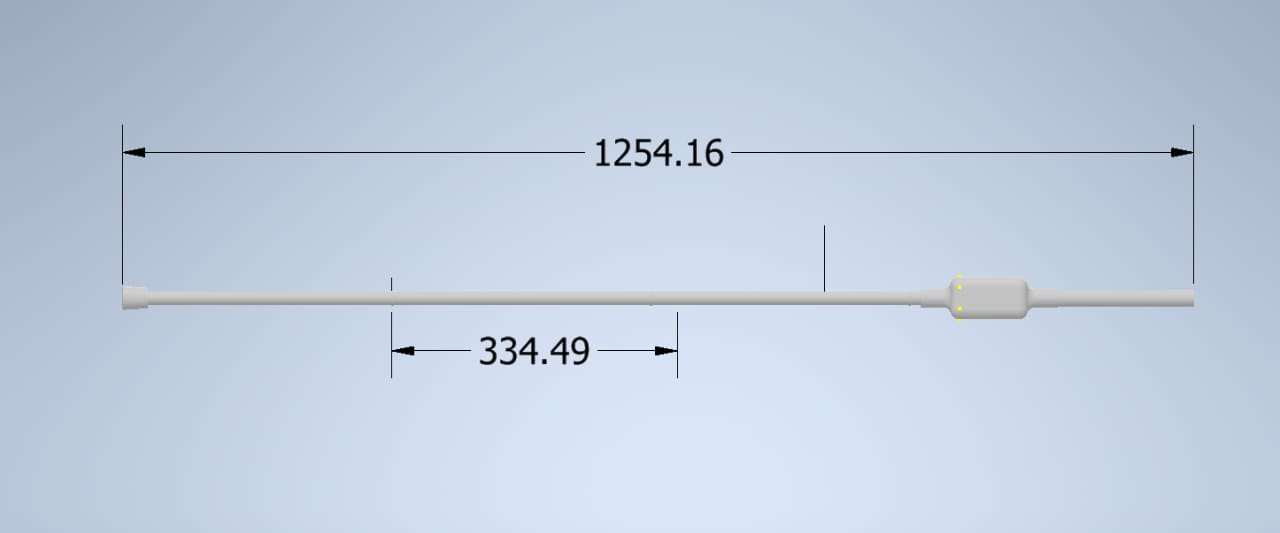
\includegraphics[width=0.7\textwidth]{figuras/prototipo1.jpeg} 
        \caption*{Fonte: eladorada pelo autor.}
    \end{figure}

    \begin{figure}[h!]
        \captionsetup{width=1\textwidth}
        \caption{\label{fig:prototipo2} Visão superior do protótipo}
        \centering
        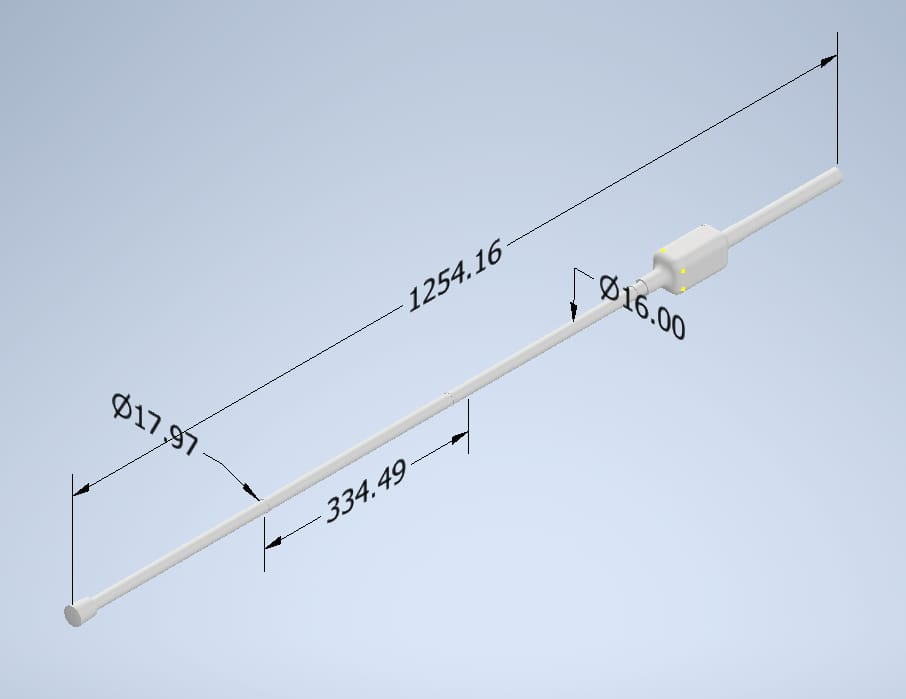
\includegraphics[width=0.7\textwidth]{figuras/prototipo2.jpeg} 
        \caption*{Fonte: eladorada pelo autor.}
    \end{figure}

        \begin{figure}[h!]
        \captionsetup{width=1\textwidth}
        \caption{\label{fig:prototipo3}Detalhamento do espaço para os componentes}
        \centering
        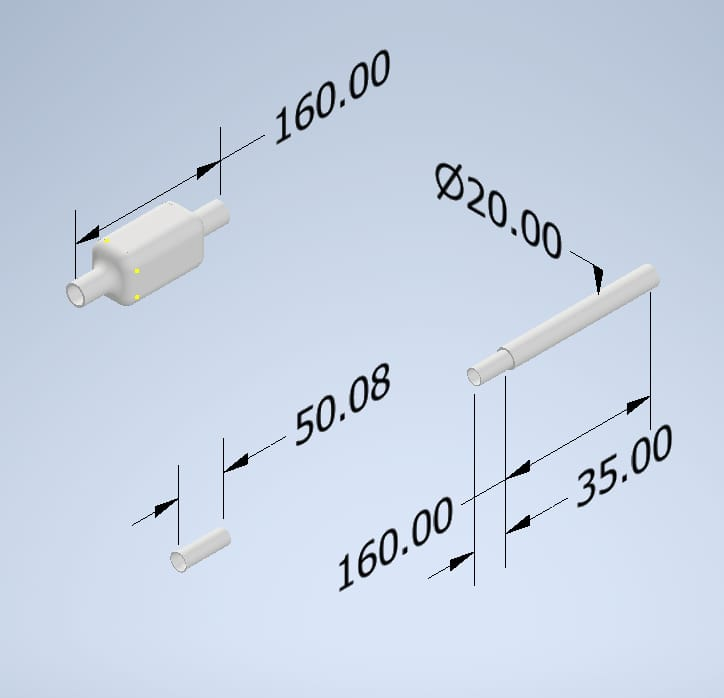
\includegraphics[width=0.7\textwidth]{figuras/prototipo3.jpeg} 
        \caption*{Fonte: eladorada pelo autor.}
    \end{figure}